\documentclass[12pt,twoside]{article}
\usepackage{jmlda}
\usepackage{subfig}
%\NOREVIEWERNOTES
\title{Результаты эксперимента}
\author{Базарова Александра}
\begin{document}
\maketitle
\section{Синтетические данные}
\subsection{Концентрические окружности}
Сначала данные с небольшим шумом по всей картинке. Исходные данные:  \begin{figure}[h]
\center{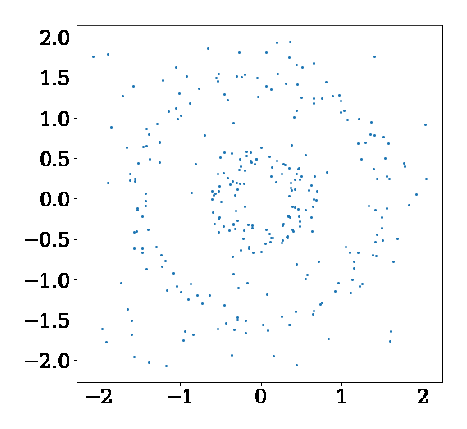
\includegraphics[scale=1]{1.eps}}
\caption{$r_0 = 0.5, \, r_1 = 1.5, \, (x_0, y_0) = (0, 0)$}
\end{figure} \\
Ответ алгоритма: \\
\begin{figure}[h]
\center{\includegraphics[scale=1]{2.eps}}
\end{figure}\\
Найденные параметры окружностей: $r_0 = 0.70, (x_0, y_0) = (0.11, 0.02); \, r_1 = 1.68, \, (x_1, y_1) = (-0.08, -0.04)$. То есть алгоритм достаточно точно восстанавливает исходные зависимости.
\newpage
Добавим шума по всей картинке: \\
\begin{figure}[h]
\center{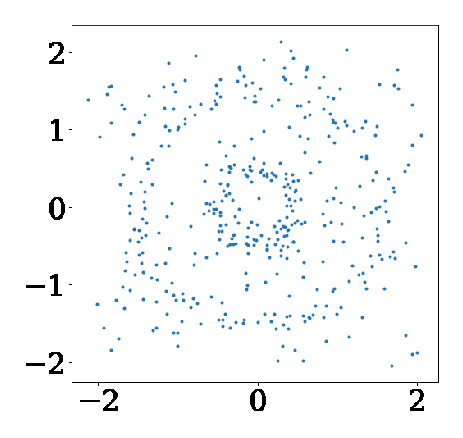
\includegraphics[scale=1]{3.eps}}
\caption{$r_0 = 0.5, \, r_1 = 1.5, \, (x_0, y_0) = (0, 0)$}
\end{figure} \\
Ответ алгоритма: \\
\begin{figure}[h]
\center{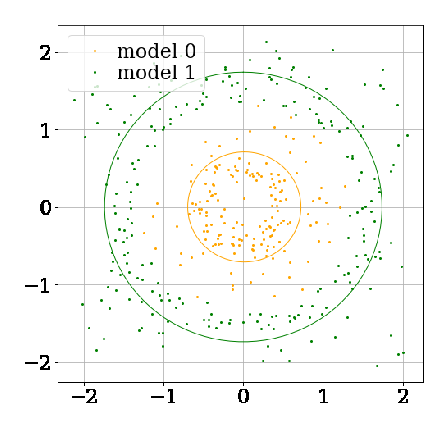
\includegraphics[scale=1]{4.eps}}
\end{figure}\\
Найденные параметры окружностей: $r_0 = 0.71, (x_0, y_0) = (0.01, -0.00); \, r_1 = 1.74, \, (x_1, y_1) = (0.00, 0.00)$.  Несмотря на увеличившийся шум, алгоритм все еще выдает неплохой результат. \newpage
\subsection{Неконцентрические окружности}
Исходные данные: \\
\begin{figure}[h]
\center{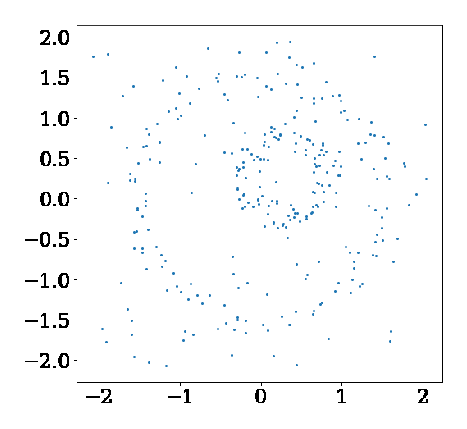
\includegraphics[scale=1]{5.eps}}
\caption{$r_0 = 0.5, \, r_1 = 1.5, \, (x_0, y_0) = (0.3, 0.3), (x_1, y_1) = (0, 0)$}
\end{figure} \\
Ответ алгоритма: $r_0 = 0.68, (x_0, y_0) = (0.18, 0.06); \, r_1 = 1.69, (x_1, y_1) = (-0.09, -0.06) $
\begin{figure}[h]
\center{\includegraphics[scale=1]{6.eps}}
\end{figure}\\
Точность нахождения окружностей снизилась.\newpage Попробуем уменьшить шум на картинке: \\
\begin{figure}[h]
\center{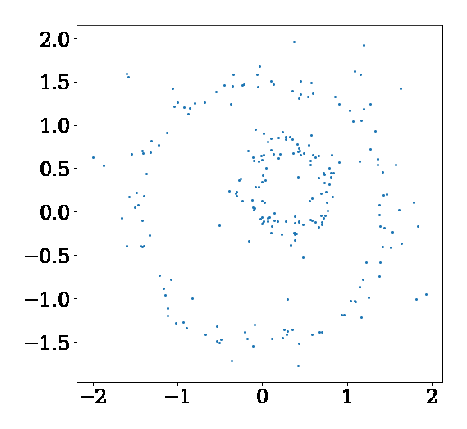
\includegraphics[scale=1]{7.eps}}
\caption{$r_0 = 0.5, \, r_1 = 1.5, \, (x_0, y_0) = (0.3, 0.3), (x_1, y_1) = (0, 0)$}
\end{figure} \\
Ответ алгоритма: \\
\begin{figure}[h]
\center{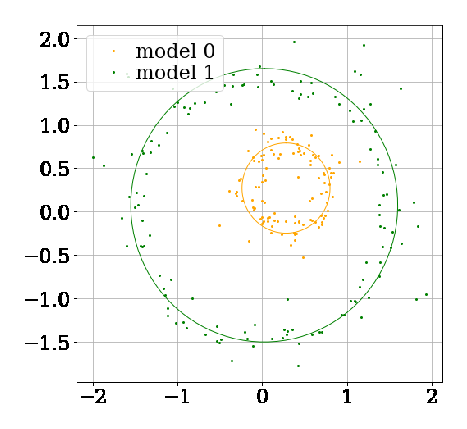
\includegraphics[scale=1]{8.eps}}
\end{figure}\\
Найденные параметры окружностей: $r_0 = 0.52, (x_0, y_0) = (0.28, 0.27); \, r_1 = 1.58, \, (x_1, y_1) = (0.02, 0.07)$. Видим, что с уменьшением равномерно распределенного по картинке шума результаты существенно улучшились. \newpage 
Расположим окружности дальше друг от друга. Сперва с незашумленной картинкой: \\
\begin{figure}[h]
\center{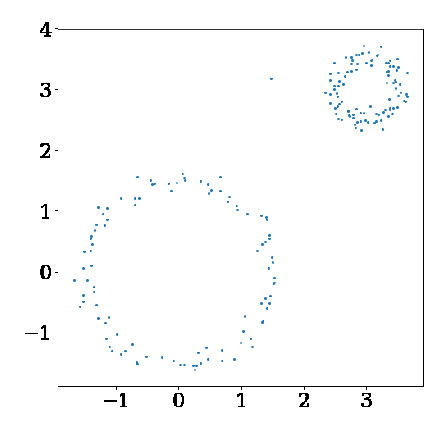
\includegraphics[scale=1]{9.eps}}
\caption{$r_0 = 0.5, \, r_1 = 1.5, \, (x_0, y_0) = (3, 3), (x_1, y_1) = (0, 0)$}
\end{figure} \\
Ответ алгоритма: \\
\begin{figure}[h]
\center{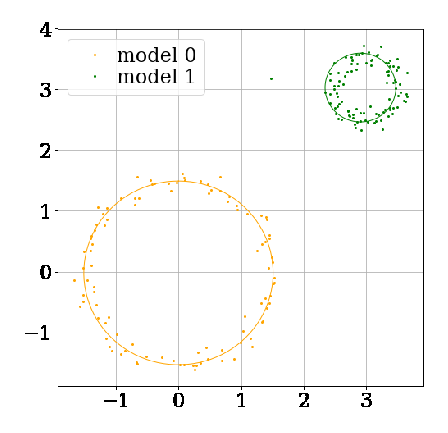
\includegraphics[scale=1]{10.eps}}
\end{figure}\\
Найденные параметры окружностей: $r_0 = 0.57, (x_0, y_0) = (2.91, 3.03); \, r_1 = 1.51, \, (x_1, y_1) = (-0.00, -0.00)$. \newpage
Добавим шум вокруг окружностей: \\
\begin{figure}[h]
\center{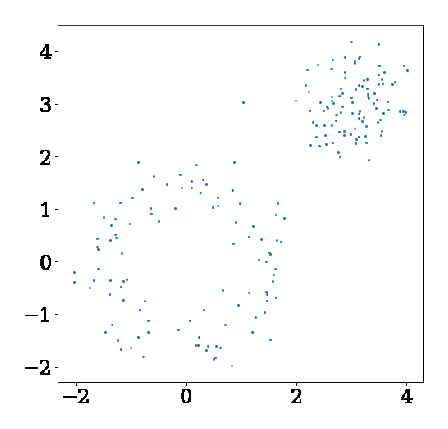
\includegraphics[scale=1]{11.eps}}
\caption{$r_0 = 0.5, \, r_1 = 1.5, \, (x_0, y_0) = (3, 3), (x_1, y_1) = (0, 0)$}
\end{figure} \\
Ответ алгоритма: \\
\begin{figure}[h]
\center{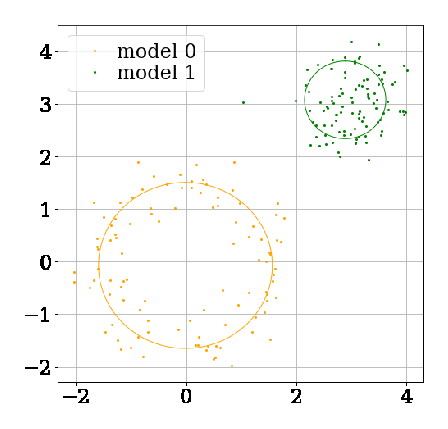
\includegraphics[scale=1]{12.eps}}
\end{figure}\\
Найденные параметры: $r_0 = 0.73, (x_0, y_0) = (2.88, 3.07); \, r_1 = 1.58, \, (x_1, y_1) = (-0.01, -0.07)$. Несмотря на шум, результаты ухудшились не сильно. \newpage
Теперь добавим совсем небольшой равномерный шум по всей картинке, уменьшив зашумленность окружностей:
\begin{figure}[h]
\center{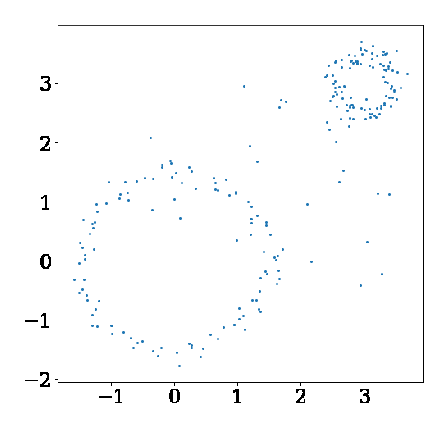
\includegraphics[scale=1]{13.eps}}
\caption{$r_0 = 0.5, \, r_1 = 1.5, \, (x_0, y_0) = (3, 3), (x_1, y_1) = (0, 0)$}
\end{figure} \\
Ответ алгоритма: \\
\begin{figure}[h]
\center{\includegraphics[scale=1]{14.eps}}
\end{figure}\\
Даже совсем небольшой шум, распределенный по картинке, <<ломает>> алгоритм.\\
Из данных выше можно сделать вывод, что наш алгоритм умеет обрабатывать <<шум каждой модели>> (зашумленность окружностей не слишком ухудшала показания алгоритма), но он пока не умеет корректно обрабатывать шум, распределенный по картинке равномерно. Необходимо создать <<модель шума>>. \\
\subsection{Три окружности}
Создадим три окружности и посмотрим, как на них работает наш алгоритм. \\
\begin{figure}[h]
\center{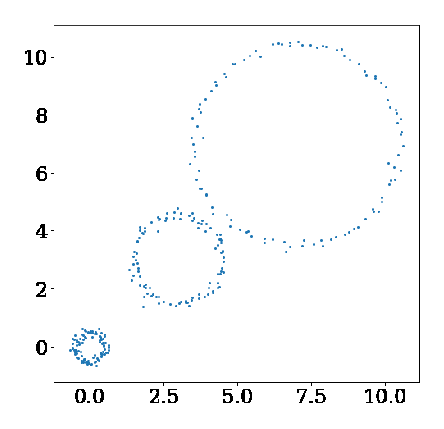
\includegraphics[scale=1]{15.eps}}
\caption{$r_0 = 0.5, \, r_1 = 1.5, r_2 = 3.5, \, (x_0, y_0) = (0, 0), (x_1, y_1) = (3, 3), (x_2, y_2) = (7, 7)$}
\end{figure} \\
Ответ алгоритма: \\
\begin{figure}[h]
\center{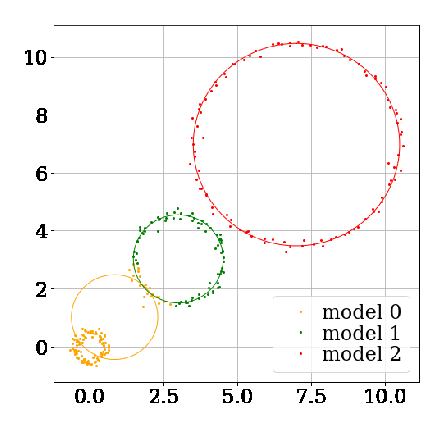
\includegraphics[scale=1]{16.eps}}
\end{figure}\\
Весьма неожиданный результат, мы видим, что одна окружность нашлась почти идеально, а две другие почему-то не были корректно отделены друг от друга. \newpage
Попробуем поменять конфигурацию: \\
\begin{figure}[h!]
\center{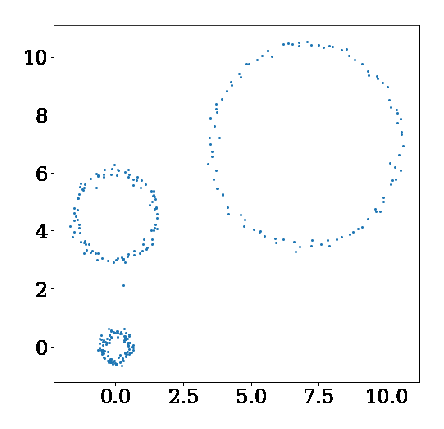
\includegraphics[scale = 0.9]{17.eps}}
\caption{$r_0 = 0.5, \, r_1 = 1.5, r_2 = 3.5, \, (x_0, y_0) = (0, 0), (x_1, y_1) = (0, 4.5), (x_2, y_2) = (7, 7)$}
\end{figure} \\ 
Ответ алгоритма: \\
\begin{figure}[h]
\center{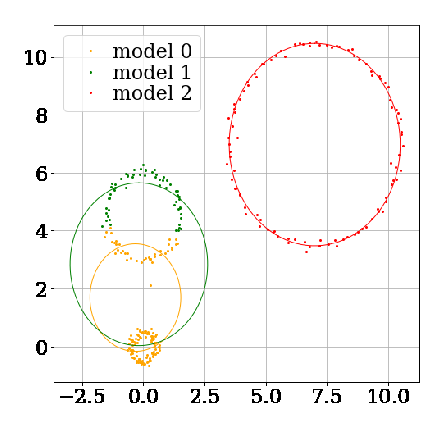
\includegraphics[scale=1]{18.eps}}
\end{figure}\\
Проблема остается все та же. \newpage Разместим окружности дальше друг от друга: 
\begin{figure}[h!]
\center{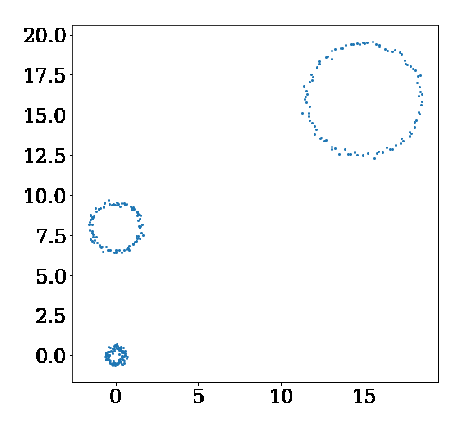
\includegraphics[scale = 0.9]{19.eps}}
\caption{$r_0 = 0.5, \, r_1 = 1.5, r_2 = 3.5, \, (x_0, y_0) = (0, 0), (x_1, y_1) = (0, 8), (x_2, y_2) = (15, 16)$}
\end{figure} \\ 
Ответ модели: \\
\begin{figure}[h]
\center{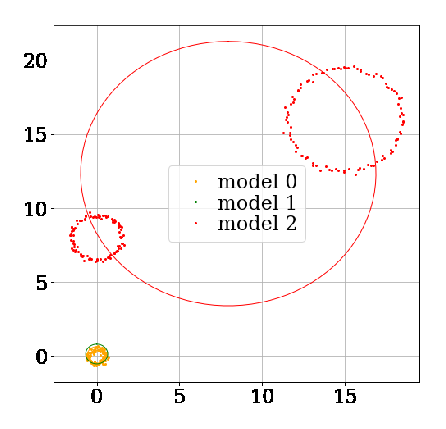
\includegraphics[scale=1]{20.eps}}
\end{figure}\\
Проблема остается. Можно понять, что она состоит не в зашумленности картинки (шум почти нулевой) и не во взаимном расположении окружностей (проблема остается и тогда, когда окружности расположены относительно далеко друг от друга). \newpage
\section{Реальные данные}
Исходная картинка: 
\begin{figure}[h]
\center{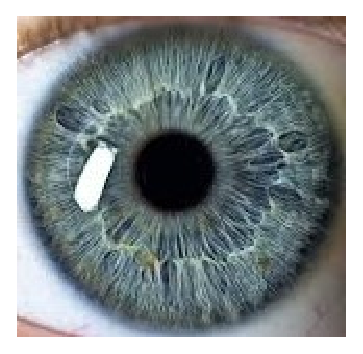
\includegraphics[scale=1]{21.eps}}
\end{figure}\\
После предобработки: \\
\begin{figure}[h]
\center{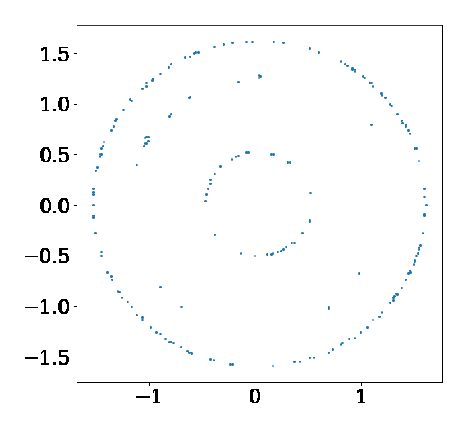
\includegraphics[scale=1]{23.eps}}
\end{figure}\\ \newpage
Видим, что тут две окружности с небольшим шумом. Посмотрим, как отработает алгоритм: \\
\begin{figure}[h]
\center{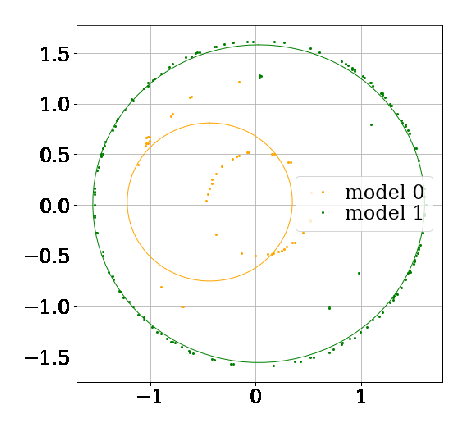
\includegraphics[scale=1]{24.eps}}
\end{figure} \\
Алгоритм неустойчив к шуму, поэтому результаты работы алгоритма не совпадают с исходными закономерностями. 
\end{document}
